\documentclass[compress]{beamer}
%\documentclass[handout,compress]{beamer}

\usepackage{bbm}
\usepackage{bm}

\newcommand{\cblue}[1]{{\color{blue}{#1}}}
\newcommand{\cgreen}[1]{{\color{green}{#1}}}

\mode<presentation> {
    \usetheme{Warsaw}
    \usecolortheme{wolverine}
    %\setbeamertemplate{footline}[page number]
    %\setbeamertemplate{footline}[frame number]

    \setbeamercovered{transparent}
    \setbeamertemplate{navigation symbols}{}% supresses navigation symbols
    \def\qedsymbol{} %supresses the \qed symbol at the end of a proof
}

\def\perc{0.57}
\def\percc{0.43}
\setbeamertemplate{footline}
{
  \leavevmode%
  \hbox{%
  \begin{beamercolorbox}[wd=\perc\paperwidth,ht=2.25ex,dp=1ex,center]{author in head/foot}%
    \usebeamerfont{author in head/foot}\insertshortauthor
  \end{beamercolorbox}%
  \begin{beamercolorbox}[wd=\percc\paperwidth,ht=2.25ex,dp=1ex,center]{title in head/foot}%
    \usebeamerfont{title in head/foot}\insertshorttitle\hspace*{1em}
    \insertframenumber{} / \inserttotalframenumber\hspace*{1ex}
  \end{beamercolorbox}}%
  \vskip0pt%
}
\makeatletter
\setbeamertemplate{headline}
{%
  \leavevmode%
  \begin{beamercolorbox}[wd=\perc\paperwidth,ht=2.5ex,dp=1.125ex]{section in head/foot}%
    \vbox to 2.5ex{\vspace{0.3ex}\insertsectionnavigationhorizontal{\perc\paperwidth}{\hskip0pt plus1filll}{}}%
  \end{beamercolorbox}%
  \begin{beamercolorbox}[wd=\percc\paperwidth,ht=2.5ex,dp=1.125ex]{subsection in head/foot}%
    \vbox to 2.5ex{\vspace{0.3ex}\insertsubsectionnavigationhorizontal{\percc\paperwidth}{}{\hskip0pt plus1filll}}%
  \end{beamercolorbox}%
}
\makeatother


\usepackage[english]{babel}
\usepackage[latin1]{inputenc}
\usepackage{times}
\usepackage[T1]{fontenc}
\usepackage{graphicx}
\usepackage{stmaryrd}
\usepackage{booktabs}
\usepackage{tikz}
\usepackage{pgfplots}
\usepackage{amssymb}
\usepackage{mathtools}
\usepackage{physymb}
\usepackage{rotating}
\usepackage{fancybox}


\def\clr{}
%\def\clr{_BW}

\newif \ifSIAM
\SIAMtrue

\newif \ifbbm
%\bbmtrue

\newif \iffract
\fracttrue

\newif \ifphysymb
\physymbtrue

\newcommand{\vertical}[1]{\begin{sideways}{#1}\end{sideways}}

%%%%%%%%%%%%%%%%%%%%%%%%%%%
% Biblio
%%%%%%%%%%%%%%%%%%%%%%%%%%%

\newcommand\subm{\rm submitted}
\newcommand\Subm{\rm Submitted}
\newcommand\submt{\rm submitted~to~}
\newcommand\Submt{\rm Submitted~to~}
\newcommand\Submfp{\rm Submitted for publication}
\newcommand\submfp{\rm submitted for publication}
\newcommand\prep{\rm In~preparation}
\newcommand\toap{\rm to~appear}
\newcommand\Afp{\rm Accepted for publication}
\newif \ifwhere
%\wheretrue
\newcommand\jour{}
%\newcommand\jour{\em}

%%%%%%%%%%%%%%%%%%%%%%%%%%%
% Environments
%%%%%%%%%%%%%%%%%%%%%%%%%%%

\newcommand{\be}{\begin{equation}}
\newcommand{\ee}{\end{equation}}
\newcommand{\bea}{\begin{eqnarray}}
\newcommand{\eea}{\end{eqnarray}}
\newcommand{\bean}{\begin{eqnarray*}}
\newcommand{\eean}{\end{eqnarray*}}
\def\ba#1\ea{\begin{align}#1\end{align}}
\def\ban#1\ean{\begin{align*}#1\end{align*}}
\def\bat#1\eat{\begin{alignat}#1\end{alignat}}
\def\batn#1\eatn{\begin{alignat*}#1\end{alignat*}}
\def\bs#1\es{\begin{split}#1\end{split}}
\newcommand{\bse}{\begin{subequations}}
\newcommand{\ese}{\end{subequations}}
\newcommand{\bt}{\begin{theorem}}
\newcommand{\et}{\end{theorem}}
\newcommand{\bl}{\begin{lemma}}
\newcommand{\el}{\end{lemma}}
\newcommand{\bc}{\begin{corollary}}
\newcommand{\ec}{\end{corollary}}
\newcommand{\bp}{\begin{proof}}
\newcommand{\ep}{\end{proof}}
\newcommand{\bd}{\begin{definition}}
\newcommand{\ed}{\end{definition}}
\newcommand{\br}{\begin{remark}}
\newcommand{\er}{\end{remark}}
\newcommand{\bas}{\begin{assumption}}
\newcommand{\eas}{\end{assumption}}
\newcommand{\bex}{\begin{example}}
\newcommand{\eex}{\end{example}}
\newcommand{\bqo}{\begin{quote}}
\newcommand{\eqo}{\end{quote}}
\newcommand{\bdc}{\begin{description}}
\newcommand{\edc}{\end{description}}
\newcommand{\bi}{\begin{itemize}}
\newcommand{\ei}{\end{itemize}}
\newcommand{\ben}{\begin{enumerate}}
\newcommand{\een}{\end{enumerate}}

\ifSIAM
\newtheorem{remark}[theorem]{Remark}
\newtheorem{assumption}[theorem]{Assumption}

\else

\newtheorem{lemma}{Lemma}[section]
\newtheorem{corollary}[lemma]{Corollary}
\newtheorem{assumption}[lemma]{Assumption}
\newtheorem{theorem}[lemma]{Theorem}
\newtheorem{definition}[lemma]{Definition}
\newtheorem{remark}[lemma]{Remark}
\newtheorem{example}[lemma]{Example}
\newtheorem{algorithm}[lemma]{Algorithm}

\fi


%%%%%%%%%%%%%%%%%%%%%%%%%%%
% Comments
%%%%%%%%%%%%%%%%%%%%%%%%%%%

% \ifbbm two versions of fonts for tensors
% \iffract fractions as 1/2 or \frac 1 2
% \Xv vector version of X
% \Xm matrix version of X
% \Xi[1] X with superscript as argument
% \tX bold X

%%%%%%%%%%%%%%%%%%%%%%%%%%%
% Domains
%%%%%%%%%%%%%%%%%%%%%%%%%%%

\newcommand\Om{\Omega}
\newcommand\om{\omega}
\newcommand\oma{{\omega_\ver}}
\newcommand{\TF}{T}
\newcommand\GD{\Gamma_{\mathrm D}}
\newcommand\GN{\Gamma_{\mathrm N}}
\newcommand\GR{\Gamma_{\mathrm R}}

%%%%%%%%%%%%%%%%%%%%%%%%%%%
% Operators
%%%%%%%%%%%%%%%%%%%%%%%%%%%

\newcommand\Gr{\nabla}
\newcommand\Grb{\nabla}
\newcommand\Dv{\nabla {\cdot}}
\newcommand\Dvb{\nabla_{\mathcal{T}} {\cdot}}
\newcommand\Crl{\nabla {\times}}
\newcommand\Rt{\Rm\nabla}
\newcommand\Rm{{\rm R}_{\frac{\pi}{2}}}
\newcommand\Rmat{\begin{pmatrix}
   0 & -1 \\
   1 & 0
  \end{pmatrix}}
\newcommand\gr{\mathrm{grad}}
\newcommand\dv{\mathrm{div}}
\newcommand\rt{\mathrm{rot}}
\newcommand\crl{\mathrm{curl}}
\newcommand\scp{{\cdot}}
\newcommand\scpm{{:}}
\newcommand\Lap{\Delta}
\newcommand\Lapb{\Delta}
\newcommand{\jump}[1]{[\![#1]\!]}
\newcommand{\aver}[1]{\{\!\!\{#1\}\!\!\}}
\renewcommand{\vec}[1]{#1}
\newcommand{\matr}[1]{\mathbb{#1}}
\newcommand\il{|\hspace{-0.02cm}|\hspace{-0.02cm}|}
\newcommand{\en}[1]{\il#1\il}
\newcommand{\ena}[1]{\il#1\il_\oplus}
\newcommand\BS{\mathcal{B}_{\mathrm{S}}}
\newcommand\BA{\mathcal{B}_{\mathrm{A}}}
\newcommand\BD{\mathcal{B}_{\mathrm{D}}}
\newcommand\bA{b_{\mathrm{A}}}

\ifbbm

\newcommand\II{{\mathbbm I}}
\newcommand{\svg}[1]{{\mathbbm d}(#1)}

\else

\newcommand\II{\underline{\bm I}}
\newcommand{\svg}[1]{\underline{\bm d}(#1)}

\fi

%%%%%%%%%%%%%%%%%%%%%%%%%%%
% Spaces
%%%%%%%%%%%%%%%%%%%%%%%%%%%

\newcommand\Ho{H^1(\Om)}
\newcommand\Hoi[1]{H^1(#1)}
\newcommand\Hoo{H^1_0(\Om)}
\newcommand\Hooi[1]{H^1_0(#1)}
\newcommand\Hmo{H^{-1}(\Om)}
\newcommand\HTh{H^1(\Th)}
\newcommand\HG{H^{1/2}(\pt \Om)}
\newcommand\Hsa{H^1_*(\oma)}
\newcommand\HTa{H^1(\Ta)}
\newcommand\Hs{H^1_*(\om)}
\newcommand\Hbsa{\bar H^1_*(\oma)}

\newcommand\Woinf{W^{1,\infty}(\Om)}
\newcommand\Wop{W^{1,p}(\Om)}
\newcommand\Wopi[1]{W^{1,p}(#1)}
\newcommand\Woop{{W^{1,p}_0(\Om)}}

\newcommand\Lt{L^2(\Om)}
\newcommand\Lti[1]{L^2(#1)}
\newcommand\Lto{L^2_0(\Om)}
\newcommand\Linf{L^\infty(\Om)}
\newcommand\Lq{L^q(\Om)}
\newcommand\Lqo{L^q_0(\Om)}
\newcommand\LtQ{L^2(\Omega \times (0,\TF))}
\newcommand\Ls{L^2_*(\oma)}
\newcommand\tLti[1]{\tL^2(#1)}

\newcommand\Cz{C^0(\overline\Om)}
\newcommand\Ct{C^2(\overline\Om)}
\newcommand\Cinf{C^\infty(\overline\Om)}
\newcommand\Do{{\mathcal D}(\Om)}
\newcommand\Doi[1]{{\mathcal D}(#1)}

\newcommand\Hdv{\tH(\dv,\Om)}
\newcommand\Hdvi[1]{\tH(\dv,#1)}
\newcommand\Hdvs{\tH_0(\dv,\oma)}
\newcommand\Hdvss{\tH^0(\dv,\oma)}
\newcommand\HdvTa{\tH(\dv,\Ta)}


%%%%%%%%%%%%%%%%%%%%%%%%%%%
% Shorthands
%%%%%%%%%%%%%%%%%%%%%%%%%%%

\newcommand\ie{i.e.}
\newcommand\eg{e.g.}
\newcommand\cf{cf.}
\newcommand\eal{{\em et al.}}
\newcommand\eq{:=}
\newcommand\qe{=:}
\newcommand\ls{\lesssim}
\newcommand\ds{\displaystyle}
\newcommand\nn{\nonumber}
\newcommand\pt{\partial}
\newcommand{\<}{\langle}
\renewcommand{\>}{\rangle}
\newcommand\ra{\rightarrow}
\newcommand\lra{\longrightarrow}
\newcommand{\sumN}{\sum_{n=1}^N}
\newcommand{\iIn}{\int_{I_n}}
\newcommand\ON{\{1, \ldots, N\}}
\newcommand\nv{0}
\newcommand\nvv{{\bm 0}}

%%%%%%%%%%%%%%%%%%%%%%%%%%%
% Meshes
%%%%%%%%%%%%%%%%%%%%%%%%%%%

\newcommand{\elm}{{K}}
\newcommand{\elmt}{{K'}}
\newcommand{\sd}{{F}}
\newcommand{\sdt}{{F'}}
\newcommand{\ver}{{\ta}}
\newcommand{\vertt}{{\ta'}}
\newcommand{\htt}{{h\tau}}

\newcommand\Fh{\mathcal{F}_h}
\newcommand\Fhint{\Fh^{\mathrm{s}}}
\newcommand\Fhext{\Fh^{\mathrm{b}}}
\newcommand\FK{\mathcal{F}_\elm}
\newcommand\FKi{\mathcal{F}_{\elm_i}}
\newcommand\FKj{\mathcal{F}_{\elm_j}}
\newcommand\Fa{\mathcal{F}_{\ver}}
\newcommand\Fas{{\Fa^{\mathrm{s}}}}
\newcommand\Fab{{\Fa^{\mathrm{b}}}}
\newcommand\Fapp{\Fa^{\partial}}
\newcommand\FaN{\Fa^{\mathrm{N}}}
\newcommand\FaD{\Fa^{\mathrm{D}}}
\newcommand\FKN{\FK^{\mathrm{N}}}
\newcommand\FKNi{\F_{\elm_i}^{\mathrm{N}}}
\newcommand\FKD{\FK^{\mathrm{D}}}
\newcommand\FKDi{\F_{\elm_i}^{\mathrm{D}}}
\newcommand\Fe{{\F_\edg}}

\newcommand{\edg}{{e}}
\newcommand\Ea{\mathcal{E}_{\ver}}

\newcommand\Th{\mathcal{T}_h}
\newcommand\TK{\mathcal{T}_\elm}
\newcommand\TKn{\mathfrak{T}_\elm}
\newcommand\Ta{{\mathcal{T}_{\ver}}}
\newcommand\Taint{\mathcal{T}_\ver^{\circ}}
\newcommand\Taext{\mathcal{T}_\ver^{\partial}}
\newcommand\Te{{\mathcal{T}_{\sd}}}
\newcommand\TEs{\mathcal{T}_{E\ups}}

\newcommand\Vh{\mathcal{V}_h}
\newcommand\Vhint{\mathcal{V}^{\circ}_h}
\newcommand\Vhext{\mathcal{V}^{\partial}_h}
\newcommand\VK{\mathcal{V}_\elm}
\newcommand\VEs{\mathcal{V}_{E\ups}}
\newcommand\Va{\mathcal{V}_{\ver}}
\newcommand\Vas{\mathcal{V}_{\ver\ups}}

%%%%%%%%%%%%%%%%%%%%%%%%%%%
% Variables
%%%%%%%%%%%%%%%%%%%%%%%%%%%

\newcommand\uu{u}
\newcommand\uh{u_h}
\newcommand\buh{{\bar u}_h}
\newcommand\uht{u_{\htt}}
\newcommand\uhtn{u_h^n}
\newcommand\uv{\tu}
\newcommand\uvh{\tu_h}
\newcommand\fh{\tp_h}

\newcommand\pr{s}
\newcommand\prh{s_h}
\newcommand\prv{\ts}
\newcommand\prhv{\ts_h}
\newcommand\prht{s_\htt}
\newcommand\prhn{s_h^n}
\newcommand\prho{s_h^0}

\newcommand\fr{{\bm \sigma}}
\newcommand\frh{{\bm \sigma}_h}
\newcommand\fro{\sigma}
\newcommand\frho{\sigma_h}
\newcommand\vfr{{\bm \varsigma}}
\newcommand\vfrh{{\bm \varsigma}_h}
\newcommand\vfrp{{\bm \varsigma}_p}

\ifbbm

%\mathbbm \mathbbmss \mathbbmtt

\newcommand\frm{{\mathbbm w}}
\newcommand\frhm{{\mathbbm w}_h}
\newcommand\frhtm{{\mathbbm w}_{\htt}}
\newcommand\Km{{\mathbbm K}}

\else

\newcommand\frm{\underline{\bm \sigma}}
\newcommand\frhm{\underline{\bm \sigma}_h}
\newcommand\frhtm{\underline{\bm \sigma}_{\htt}}
\newcommand\Km{\underline{\bf K}}

\fi

%%%%%%%%%%%%%%%%%%%%%%%%%%%
% Estimators
%%%%%%%%%%%%%%%%%%%%%%%%%%%

\newcommand\eelm{\eta_{\elm}}
\newcommand\eelmi[1]{\eta_{\elm}^{#1}}
\newcommand\eA{\eta}
\newcommand\eAi[1]{\eta^{#1}}

\newcommand\eres{\eta_{\mathrm{R},\elm}}
\newcommand\eresi[1]{\eta_{\mathrm{R},\elm}^{#1}}
\newcommand\eresA{\eta_{\mathrm{R}}}
\newcommand\eresAi[1]{\eta_{\mathrm{R}}^{#1}}

\newcommand\ef{\eta_{\mathrm{F},\elm}}
\newcommand\efi[1]{\eta_{\mathrm{F},\elm}^{#1}}
\newcommand\efii[2]{\eta_{\mathrm{F},#1,\elm}^{#2}}
\newcommand\efA{\eta_{\mathrm{F}}}
\newcommand\efAi[1]{\eta_{\mathrm{F}}^{#1}}

\newcommand\enc{\eta_{\mathrm{NC},\elm}}
\newcommand\enci[1]{\eta_{\mathrm{NC},\elm}^{#1}}
\newcommand\encii[2]{\eta_{\mathrm{NC},#1,\elm}^{#2}}
\newcommand\encA{\eta_{\mathrm{NC}}}
\newcommand\encAi[1]{\eta_{\mathrm{NC}}^{#1}}
\newcommand\tenc{\widetilde\eta_{\mathrm{NC},\elm}}
\newcommand\tenci[1]{\widetilde\eta_{\mathrm{NC},#1,\elm}}

\newcommand\edisc{\eta_{\mathrm{disc},\elm}}
\newcommand\edisci[1]{\eta_{\mathrm{disc},\elm}^{#1}}
\newcommand\ediscA{\eta_{\mathrm{disc}}}
\newcommand\ediscAi[1]{\eta_{\mathrm{disc}}^{#1}}

\newcommand\elin{\eta_{\mathrm{lin},\elm}}
\newcommand\elini[1]{\eta_{\mathrm{lin},\elm}^{#1}}
\newcommand\elinA{\eta_{\mathrm{lin}}}
\newcommand\elinAi[1]{\eta_{\mathrm{lin}}^{#1}}

\newcommand\eae{\eta_{\mathrm{alg},\elm}}
\newcommand\eaei[1]{\eta_{\mathrm{alg},\elm}^{#1}}
\newcommand\eaeA{\eta_{\mathrm{alg}}}
\newcommand\eaeAi[1]{\eta_{\mathrm{alg}}^{#1}}

\newcommand\ereg{\eta_{\mathrm{reg},\elm}}
\newcommand\eregi[1]{\eta_{\mathrm{reg},\elm}^{#1}}
\newcommand\eregA{\eta_{\mathrm{reg}}}
\newcommand\eregAi[1]{\eta_{\mathrm{reg}}^{#1}}

\newcommand\eosc{\eta_{\mathrm{osc},\elm}}
\newcommand\eosci[1]{\eta_{\mathrm{osc},\elm}^{#1}}
\newcommand\eoscA{\eta_{\mathrm{osc}}}
\newcommand\eoscAi[1]{\eta_{\mathrm{osc}}^{#1}}

\newcommand\erem{\eta_{\mathrm{rem},\elm}}
\newcommand\eremi[1]{\eta_{\mathrm{rem},\elm}^{#1}}
\newcommand\eremA{\eta_{\mathrm{rem}}}
\newcommand\eremAi[1]{\eta_{\mathrm{rem}}^{#1}}

\newcommand\eclas{\eta_{\mathrm{\sharp},\elm}}
\newcommand\eclasA{\eta_{\mathrm{\sharp}}}

\newcommand\epot{\eta_{\mathrm{P},\elm}}

\newcommand\ediv{\eta_{\mathrm{D},\elm}}
\newcommand\edivi[1]{\eta_{\mathrm{D},\elm}^{#1}}
\newcommand\edivA{\eta_{\mathrm{D}}}
\newcommand\edivAi[1]{\eta_{\mathrm{D}}^{#1}}

\newcommand\esp{\eta_{\mathrm{sp},\elm}}
\newcommand\espi[1]{\eta_{\mathrm{sp},\elm}^{#1}}
\newcommand\espii[2]{\eta_{\mathrm{sp},#1}^{#2}}
\newcommand\espA{\eta_{\mathrm{sp}}}
\newcommand\espAi[1]{\eta_{\mathrm{sp}}^{#1}}

\newcommand\etm{\eta_{\mathrm{tm},\elm}}
\newcommand\etmi[1]{\eta_{\mathrm{tm},\elm}^{#1}}
\newcommand\etmA{\eta_{\mathrm{tm}}}
\newcommand\etmAi[1]{\eta_{\mathrm{tm}}^{#1}}

\newcommand\Eic{\eta_{\mathrm{IC}}}

\newcommand{\Res}{\mathcal{R}}
\newcommand\Ieff{I_{\mathrm{eff}}}

\newcommand\eaeAA{\eta_{\mathrm{AE}}}
\newcommand\eaeAt{\hat\eta_{\mathrm{AE}}}

%%%%%%%%%%%%%%%%%%%%%%%%%%%
% Greek letters
%%%%%%%%%%%%%%%%%%%%%%%%%%%

\newcommand\al{\alpha}
\newcommand\vf{\varphi}
\newcommand\ve{\varepsilon}
\newcommand\sg{\sigma}

%%%%%%%%%%%%%%%%%%%%%%%%%%%
% Bold letters arabic
%%%%%%%%%%%%%%%%%%%%%%%%%%%

\newcommand\ta{{\bm a}}
\newcommand\tb{{\bm b}}
\newcommand\tc{{\bm c}}
\newcommand\te{{\bm e}}
\newcommand\tf{{\bm f}}
\newcommand\ti{{\bm i}}
\newcommand\tl{{\bm l}}
\newcommand\tm{{\bm m}}
\newcommand\tn{{\bm n}}
\newcommand\tp{{\bm p}}
\newcommand\tq{{\bm q}}
\newcommand\tr{{\bm r}}
\newcommand\ts{{\bm s}}
\newcommand\ttt{{\bm t}}
\newcommand\tu{{\bm u}}
\newcommand\tv{{\bm v}}
\newcommand\tw{{\bm w}}
\newcommand\tx{{\bm x}}
\newcommand\ty{{\bm y}}
\newcommand\tz{{\bm z}}

\newcommand\tA{{\bm A}}
\newcommand\tC{{\bm C}}
\newcommand\tD{{\bm D}}
\newcommand\tE{{\bm E}}
\newcommand\tF{{\bm F}}
\newcommand\tG{{\bm G}}
\newcommand\tH{{\bm H}}
\newcommand\tI{{\bm I}}
\newcommand\tK{{\bm K}}
\newcommand\tL{{\bm L}}
\newcommand\tM{{\bm M}}
\newcommand\tN{{\bm N}}
\newcommand\tP{{\bm P}}
\newcommand\tQ{{\bm Q}}
\newcommand\tR{{\bm R}}
\newcommand\tS{{\bm S}}
\newcommand\tT{{\bm T}}
\newcommand\tU{{\bm U}}
\newcommand\tV{{\bm V}}
\newcommand\tW{{\bm W}}
\newcommand\tX{{\bm X}}
\newcommand\tZ{{\bm Z}}

%%%%%%%%%%%%%%%%%%%%%%%%%%%
% Bold Greek letters
%%%%%%%%%%%%%%%%%%%%%%%%%%%

\newcommand{\bsig}{\overline{\bm \sigma}}
\newcommand{\bxi}{{\bm\xi}}
\newcommand\bvf{{\bm \varphi}}
\newcommand\bphi{{\bm \phi}}
\newcommand\bpsi{{\bm \psi}}
\newcommand\btau{{\bm \tau}}

%%%%%%%%%%%%%%%%%%%%%%%%%%%
% Mathcal letters
%%%%%%%%%%%%%%%%%%%%%%%%%%%

\newcommand\A{\mathcal{A}}
\newcommand\B{\mathcal{B}}
\newcommand\C{\mathcal{C}}
\newcommand\D{\mathcal{D}}
\newcommand\E{\mathcal{E}}
\newcommand\F{\mathcal{F}}
\newcommand\G{\mathcal{G}}
\newcommand\I{\mathcal{I}}
\newcommand\J{\mathcal{J}}
\newcommand\K{\mathcal{K}}
\newcommand\M{\mathcal{M}}
\newcommand\N{\mathcal{N}}
%\newcommand\O{\mathcal{O}}
%\newcommand\P{\mathcal{P}}
\newcommand\Q{\mathcal{Q}}
\newcommand\R{\mathcal{R}}
%\newcommand\S{\mathcal{S}}
\newcommand\T{\mathcal{T}}
\newcommand\X{\mathcal{X}}
\newcommand\Y{\mathcal{Y}}
\newcommand\V{\mathcal{V}}

%%%%%%%%%%%%%%%%%%%%%%%%%%%
% Polynomial spaces
%%%%%%%%%%%%%%%%%%%%%%%%%%%

\newcommand\RR{{\mathbb R}}
\newcommand\NN{{\mathbb N}}

\newcommand\PP{{\mathbb P}}
\newcommand\QQ{{\mathbb Q}}

\newcommand\RT{{\mathbbm{RT}}}
\newcommand\RTN{\bm{RTN}}



%%%%%%%%%%%%%%%%%%%%%%%%%%%
% Subscripts and superscripts
%%%%%%%%%%%%%%%%%%%%%%%%%%%

\newcommand\ro{\mathrm{o}}
\newcommand\rw{\mathrm{w}}
\newcommand\out{\mathrm{out}}
\newcommand\inp{\mathrm{in}}

%%%%%%%%%%%%%%%%%%%%%%%%%%%
% Fractions
%%%%%%%%%%%%%%%%%%%%%%%%%%%

\iffract

\newcommand\ft{{\frac 1 2}}
\newcommand\mft{{-\frac 1 2}}
\newcommand\fq{{\frac 1 q}}

\else

\newcommand\ft{{1/2}}
\newcommand\mft{{-1/2}}
\newcommand\fq{{1/q}}

\fi

\newcommand{\tft}{{\tfrac{1}{2}}}
\newcommand{\mtft}{{-\tfrac{1}{2}}}

%%%%%%%%%%%%%%%%%%%%%%%%%%%
% Projections
%%%%%%%%%%%%%%%%%%%%%%%%%%%

\newcommand\PIn{\mathcal{P}_{I_n}}
\newcommand\QIn{\mathcal{Q}_{I_n}}
\newcommand\Iav{\mathcal{I}_{\mathrm{av}}}
\newcommand\IV{I_{\tV_h}}

%%%%%%%%%%%%%%%%%%%%%%%%%%%
% Integration
%%%%%%%%%%%%%%%%%%%%%%%%%%%

\newcommand\dx{\, \mathrm{d} \tx}
\newcommand\dy{\, \mathrm{d} \ty}
\newcommand\dxx{\, \mathrm{d} x}
\newcommand\dyy{\, \mathrm{d} y}
\newcommand\dzz{\, \mathrm{d} z}
\newcommand\dxo{\, \mathrm{d} x_1}
\newcommand\dxt{\, \mathrm{d} x_2}
\newcommand\dxr{\, \mathrm{d} x_3}
\newcommand\dgx{\, \mathrm{d} \gamma(\tx)}
\newcommand\dgy{\, \mathrm{d} \gamma(\ty)}
\newcommand\dS{\, \mathrm{d} S}
\newcommand\dt{\, \mathrm{d} t}
\newcommand\dss{\, \mathrm{d} s}
\newcommand\dtau{\, \mathrm{d} \tau}

%%%%%%%%%%%%%%%%%%%%%%%%%%%
% Constants
%%%%%%%%%%%%%%%%%%%%%%%%%%%

\newcommand\cKK{c_{\Km, \elm}}

\newcommand{\upv}{^\mathrm{v}}
\newcommand{\ups}{^\mathrm{s}}
\newcommand{\upb}{^\mathrm{b}}
\newcommand{\dK}{\partial \elm}


\newtheorem{assumptionA}{Assumption~A}
\newtheorem{assumptionB}{Assumption~B}
\newtheorem{assumptionC}{Assumption~C}

\tabcolsep 2pt

\logo{\vspace*{-0.3cm}
\includegraphics[height=0.85cm]{INRIA-SCIENTIFIQUE-UK-RVB.jpg}\hspace*{-0.1cm}
\includegraphics[height=1cm]{ERC.jpg}}

\title[Stable broken $H^1$ \!\!\! \& ${\bf H}(\mathrm{div})$ polynomial extensions\!\!\!\!]
{Stable broken $H^1$ and ${\bf H}(\mathrm{div})$ polynomial extensions}

\author[A. Ern, \underline{M. Vohral\'\i k}]
{{\bf Alexandre Ern, \underline{Martin Vohral\'\i k}}}

\institute[Inria Paris] {
    {\em Inria Paris}}

\date[Oberwolfach, September 22, 2016] % (optional, should be abbreviation of conference name)
{Oberwolfach, September 22, 2016}

\subject{Numerical analysis}% PDF information catalog

\AtBeginSection[] {
    \begin{frame}<beamer>[noframenumbering]
        \frametitle{Outline}
        \tableofcontents[currentsection]
    \end{frame}
}
\AtBeginSubsection[] {
    \begin{frame}<beamer>[noframenumbering]
        \frametitle{Outline}
        \tableofcontents[currentsection,currentsubsection]
    \end{frame}
}

\begin{document}

\frame[plain]{\titlepage}

\begin{frame}<beamer>[noframenumbering]
    \frametitle{Outline}
    \tableofcontents
\end{frame}


\section[Results \& applications]{Main results \& applications}

\begin{frame}
\frametitle{Literature}

{\bf Fundamental results on a reference tetrahedron}

\bi

\item Costabel \& McIntosh (2010): bounded right inverse of the divergence
operator for polynomial volume data

\item Demkowicz, Gopalakrishnan, Sch{\"o}berl (2009, 2012): polynomial
extensions in $H^1$ and ${\bf H}(\mathrm{div})$ for polynomial boundary data

\ei

\pause

{\bf Stable broken ${\bf H}(\mathrm{div})$ polynomial extension on a patch}

\bi

\item Braess, Pillwein, \& Sch{\"o}berl (2009), 2D

\item volume and boundary data

\ei

\pause

{\bf Stable broken $H^1$ polynomial extensions on a patch}

\bi

\item Ern \& V. (2015), 2D, by rotation from the result of Braess, Pillwein,
\& Sch{\"o}berl

\item only boundary data (divergence-free vectors are curls)

\ei

\end{frame}


\begin{frame}
\frametitle{Setting}

%\hspace*{3cm}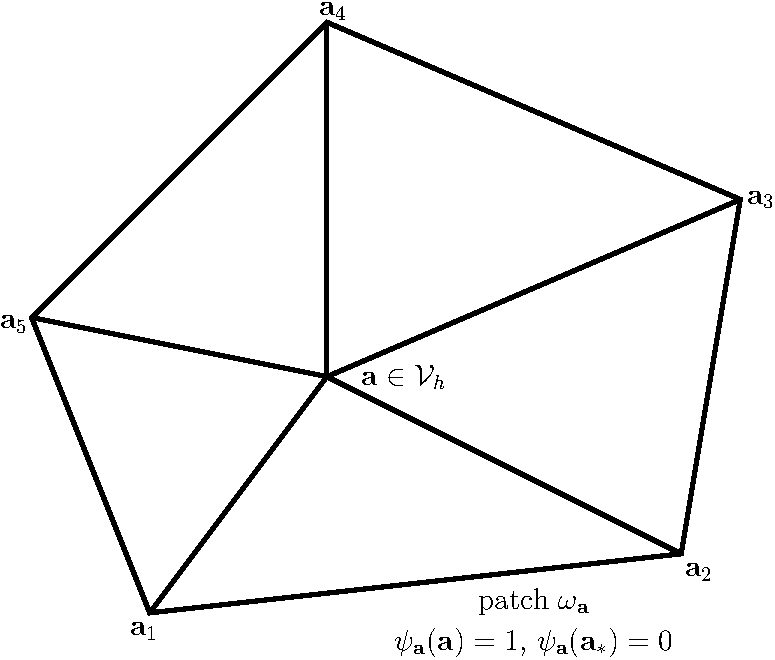
\includegraphics[height=3.5cm]{patch.pdf}

%\vspace*{-0.7cm}

{\bf Patches}

\bi

\item $\Ta\subset\Th$: patch of elements sharing $\ver \in \Vh$, subdomain
$\oma$

\item $\Fa = \Fas\cup\Fab$: faces of the elements in the patch $\Ta$, $\ver
\in \Vhint$
%(skeleton \& boundary)

\ei

\pause

{\bf Piecewise $H^1$ spaces}
%
\vspace*{-0.2cm}
%
\ban
    \HTa & \eq \{v \in \Lti{\oma}; \, v|_\elm \in \Hoi{\elm} \quad \forall \elm
    \in \Ta\}%,\\
    %\Hsa & \eq \{v \in \Hoi{\oma}; \, (v, 1)_\oma = 0\} \text{ for } \ver \in
    %\Vhint
\ean

\pause

{\bf Piecewise $\tH(\dv)$ spaces}
%
\vspace*{-0.2cm}
%
\ban
    \HdvTa & \eq \{\tv \in \tLti{\oma}; \, \tv|_\elm \in \Hdvi{\elm} \quad
    \forall \elm \in\Ta\}%,\\
    %\Hdvs & \eq \{\tv \in \Hdvi{\oma}; \, \tv \scp \tn_\oma = 0 \text{ on }
    %\pt \oma\}\text{ for } \ver \in \Vhint
\ean


\end{frame}

\begin{frame}
\frametitle{Main result: potentials}

\bt[Broken $H^1$ polynomial extension; {\scriptsize Ern \& V. (2015) in 2D}]
\label{thm_H1_ext} For $p \ge 1$ and $\ver \in \Vhint$, let $\alert{r \in
\PP_{p}(\Fas)}$. Suppose the \cblue{compatibility}
%
\batn{2}
    r & = 0 \qquad & & \text{on } \pt \oma, \\
    \sum_{\sd \in \Fe} \iota_{\sd, \edg} \, r_\sd|_\edg & = 0 & &  \forall \edg \in \Ea.
\eatn
%
Then there exists a constant $C_{\rm st} > 0$ only depending on the mesh
\cblue{shape-regularity} parameter $\kappa_{\Th}$ such that
%
\[
    \min_{\substack{v_h \in \alert{\PP_p(\Ta)}\\
    v_h = 0 \text{ on } \pt \oma,\\
    \jump{v_h} = r_\sd \,\, \forall \sd \in \Fas}} \norm{\Grb v_h}_\oma
    \alert{\leq C_{\rm st}} \min_{\substack{v \in \alert{\HTa}\\
    v = 0 \text{ on } \pt \oma,\\
    \jump{v} = r_\sd \,\, \forall \sd \in \Fas}} \norm{\Grb v}_\oma.
\]
%
\et

\end{frame}

\begin{frame}
\frametitle{Main result: fluxes}

\bt[Broken $\tH(\dv)$ polynomial extension; {\scriptsize Braess, Pillwein, \&
Sch{\"o}berl (2009) in 2D}] \label{thm_Hdv_ext} For $p \ge 1$ and $\ver \in
\Vhint$, let $\alert{r \in \PP_{p}(\Fa) \times \PP_p(\Ta)}$. Suppose the
\cblue{compatibility}
%
\[
    \sum_{\elm \in \Ta} (r_\elm, 1)_\elm - \sum_{\sd \in
    \Fa} (r_\sd, 1)_\sd = 0.
\]
%
Then there exists a constant $C_{\rm st} > 0$ only depending on the
\cblue{shape-regularity} parameter $\kappa_{\Th}$ such that
%
\[
    \min_{\substack{\tv_h \in \alert{\RTN_p(\Ta)}\\
    \tv_h \scp \tn_\sd = r_\sd \,\, \forall \sd \in \Fab\\
    \jump{\tv_h \scp \tn_\sd} = r_\sd \,\, \forall \sd \in \Fas\\
    \Dvb \tv_h|_\elm = r_\elm \,\, \forall \elm \in \Ta}}
    \norm{\tv_h}_\oma \alert{\leq C_{\rm st}}
    \min_{\substack{\tv \in \alert{\HdvTa}\\
    \tv \scp \tn_\sd = r_\sd \,\, \forall \sd \in \Fab\\
    \jump{\tv \scp \tn_\sd} = r_\sd \,\, \forall \sd \in \Fas\\
    \Dvb \tv|_\elm = r_\elm \,\, \forall \elm \in \Ta}}
    \norm{\tv}_\oma.
\]
%
\et

\end{frame}

\begin{frame}
\frametitle{Application to piecewise polynomial approximation}

{\bf Volume liftings}

\bi

\item $\tau_h \in \PP_p(\Ta)$ so that $\tau_h|_{\sd} = 0$ $\forall
\sd\in\F_\ver\upb$, and $\jump{\tau_h}_\sd = r_\sd$ $\forall \sd \in \Fas$

\visible<3->{\item $\btau_h \in \RTN_p(\Ta)$ so that
$\btau_h\scp\tn_\sd=r_\sd$ $\forall \sd\in\Fab$ and $\jump{\btau_h \scp
\tn_\sd} = r_\sd$ $\forall \sd \in \Fas$}

\ei

\uncover<2->{

\bc[Stability of best piecewise polynomial approximation] There holds
\ban\vspace*{-0.7cm}
    \visible<2->{\min_{v_h \in \alert{\PP_p(\Ta) \cap \Hooi{\oma}}} \norm{\Grb (\tau_h - v_h)}_\oma
    & \leq C_{\rm st}
    \min_{v \in \alert{\Hooi{\oma}}} \norm{\Grb (\tau_h - v)}_\oma,} \\
    \visible<4>{\min_{\substack{\tv_h \in \alert{\RTN_{p}(\Ta) \cap \Hdvs}\\
    \Dv \tv_h|_\elm = r_\elm - \Dvb \btau_h|_\elm\,\, \forall \elm \in \Ta}}\!\!\!\! \norm{\btau_h + \tv_h}_\oma
    & \leq C_{\rm st} \!\!\!\!\!\!\!\!\!\!
    \min_{\substack{\tv \in \alert{\Hdvs}\\
    \Dv \tv|_\elm = r_\elm - \Dvb \btau_h|_\elm\,\, \forall \elm \in \Ta}}\!\!\!\!\!\!\!\!\!\!\!\! \norm{\btau_h +
    \tv}_\oma \!.}
\ean\vspace*{-0.3cm} \ec}

\end{frame}

\begin{frame}
\frametitle{Application to a posteriori error analysis}

{\bf Laplace model problem}

For $f \in \PP_{p'-1}(\Th)$, $p' \geq 1$, find $\uu \in \Hoo$ such that
%
\[
    (\Gr \uu, \Gr v) = (f,v) \qquad \forall v \in \Hoo
\]

\pause

{\bf Approximate solution} with hat-function orthogonality

$\uh \in \PP_{p'}(\Th)$, \alert{$\uh \not \in \Hoo$}, \alert{$-\Grb \uh \not
\in \Hdv$}
%
\[
    (\Grb \uh, \Gr \psi_\ver)_\oma = (f, \psi_\ver)_\oma
    \qquad \forall \ver \in \Vhint
\]

\pause

{\bf Potential case} ($p=p'+1$)
%
\ban
    r_\sd & \eq \psi_\ver \jump{\uh}|_\sd,\\
    \tau_h & \eq \psi_\ver \uh
\ean

\pause

{\bf Flux case} ($p=p'$)
%
\ban
    r_\sd & \eq \psi_\ver \jump{\Grb \uh \scp \tn_\sd}|_\sd,\\
    r_\elm & \eq \psi_\ver (f + \Lapb \uh)|_\elm,\\
    \btau_h & \eq \psi_\ver \Grb \uh
\ean

\end{frame}

\begin{frame}
\frametitle{Potential reconstruction}

\bd[Potential reconstruction] For each $\ver \in \Vh$, let $\prh^\ver$ be
given by
%
\vspace{-0.2cm}
%
\[
    \prh^\ver \eq \arg \min_{v_h \in \PP_p(\Ta) \cap \Hooi{\oma}} \norm{\Grb (\psi_\ver \uh - v_h)}_\oma.
\]

\vspace{-0.15cm}
%
Then set $\alert{\prh \eq \sum_{\ver \in \Vh} \prh^\ver} \in \PP_{p}(\Th)
\cap \Hoo$. \ed

\pause

{\bf Equivalent form}

Find $\prh^\ver \in \PP_p(\Ta) \cap \Hooi{\oma}$ such that
%
\[
    (\Gr \prh^\ver, \Gr v_h)_\oma = (\Grb (\psi_\ver \uh), \Gr v_h)_\oma \qquad \forall v_h \in \PP_p(\Ta) \cap \Hooi{\oma}.
\]
%


\end{frame}

\begin{frame}
\frametitle{Flux reconstruction}

\bd[Flux reconstruction] For each $\ver \in \Vh$, let $\frh^\ver$ be given by
%
\vspace{-0.2cm}
%
\[
    \frh^\ver \eq \arg \min_{\substack{\tv_h \in \RTN_{p}(\Ta) \cap \Hdvs\\
    \Dv \tv_h=(\psi_\ver f - \Gr \psi_\ver \scp \Grb \uh)|_\elm \,\, \forall \elm \in \Ta}} \norm{\psi_\ver \Grb \uh + \tv_h}_\oma.
\]

\vspace{-0.15cm}
%
Then set $\alert{\frh \eq \sum_{\ver \in \Vh} \frh^\ver} \in \RTN_{p}(\Th)
\cap \Hdv$. \ed

\pause

{\bf Equivalent form}

Find $\frh^\ver \in \tV_h^\ver \eq \RTN_{p}(\Ta) \cap \Hdvs$ and $r_h^\ver
\in Q_h^\ver \eq \PP_p(\Ta)$ with mean value zero such that
%
\batn{2}
    (\frh^\ver, \tv_h)_\oma - (r_h^\ver, \Dv \tv_h)_\oma & = - (\psi_\ver \Grb \uh, \tv_h)_\oma
    & \quad & \forall \tv_h \in \tV_h^\ver, \\
    (\Dv \frh^\ver,q_h)_\oma & = (\psi_\ver f - \Gr \psi_\ver \scp \Grb \uh, q_h)_\oma & \quad &\forall q_h \in
    Q_h^\ver.
\eatn

\end{frame}

\begin{frame}
\frametitle{Guaranteed reliability and $p$-robust efficiency}

\vspace{-0.1cm}

{\bf Guaranteed \cblue{reliability}}
%
\vspace{-0.1cm}
%
\[
    \norm{\Grb(\uu - \uh)}^2 \leq \sum_{\elm \in \Th}
    \norm{\Grb \uh + \frh}_\elm^2 + \sum_{\elm \in \Th} \norm{\Grb (\uh - \prh)}_\elm^2
\]

\pause

{\bf Potential local \cblue{$p$-robust efficiency}}
%
\vspace{-0.2cm}
%
\[
    \hspace*{-0.8cm}\norm{\Grb (\psi_\ver \uh \! - \! \prh^\ver)}_\oma \!\! \leq \! C_{\rm st} C_{\rm cont, bPF} \visible<3>{\Biggl(\!\!\!}\norm{\Grb (\uu - \uh)}_\oma
    \! \visible<3>{+ \Biggl\{\!\sum_{\sd \in \Fa \setminus \Fab} \!\! h_\sd^{-1} \!\! \norm{\Pi_\sd^0 \jump{\uh}}_\sd^2\Biggr\}^\ft \Biggr)}
\]

\vspace{-0.2cm}

\uncover<4->{

{\bf Flux local \cblue{$p$-robust efficiency}}
%
\vspace{-0.1cm}
%
\[
    \norm{\psi_\ver \Grb \uh + \frh^\ver}_\oma
    \leq C_{\rm st} C_{\rm cont, PF} \norm{\Grb(\uu - \uh)}_\oma
\]}

\uncover<5->{

\vspace{-0.25cm}

{\bf Applications}

\bi

\item conforming finite elements

\item nonconforming finite elements

\item discontinuous Galerkin

\item mixed finite elements

\item \ldots

\ei }

\end{frame}

\section[Key ingredients]{Key ingredients}

\subsection[Stable polynomial extensions]{Stable polynomial extensions on a tetrahedron}

\begin{frame}
\frametitle{Potentials (following {\scriptsize Demkowicz, Gopalakrishnan,
Sch{\"o}berl (2009)})}

\bl[$H^1$ polynomial extension on a tetrahedron] Let $\elm \in \Th$,
$\alert{\FKD} \subset \FK$. Let $r \in \PP_{p}(\FKD)$ be continuous on
$\FKD$. Then for $C=C(\kappa_{\elm})
> 0$,
%
\[
    \!\visible<4->{\norm{\Gr \zeta_{h,\elm}}_\elm \! \stackrel{\text{FEs}}{=}} \!\!\!\!\!\!\!\!\!\min_{\substack{v_h \in \alert{\PP_p(\elm)}\\
    v_h = r_\sd \text{ on all } \sd \in \FKD}} \!\!\!\!\!\!\!\! \norm{\Gr v_h}_\elm
    \! \alert{\leq} \! C \!\!\!\!\! \min_{\substack{v \in \alert{\Hoi{\elm}}\\
    v = r_\sd \text{ on all } \sd \in \FKD}} \!\!\!\!\!\!\!\! \norm{\Gr v}_\elm \visible<3->{\! = \! C \norm{\Gr \zeta_\elm}_\elm}\!.
\]
%
\el

\visible<2->{ \begin{center}\ovalbox{ \begin{minipage}{0.62\textwidth} \,
{\bf Context} \vspace{-0.3cm} \batn{2}
    - \Lap \zeta_\elm & = 0 \qquad & & \mbox{ in } \, \elm, \\
    \zeta_\elm & = \alert{r_\sd} & & \mbox{ on all } \sd \in \FKD, \\
    -\Gr \zeta_\elm \scp \tn_\elm & = 0 & & \mbox{ on all } \sd \in \FK \setminus \FKD.
\eatn \end{minipage} } \end{center}}

\end{frame}

\begin{frame}
\frametitle{Fluxes (fol. {\scriptsize Costabel \& McIntosh (2010), Demkowicz,
Gopalakrishnan, Sch{\"o}berl (2012)})}

\bl[$\tH(\dv)$ polynomial extension on a tetrahedron] Let $\elm \in \Th$,
$\alert{\FKN} \subset \FK$. Let $r \in \PP_{p}(\FKN) \times \PP_{p}(\elm)$,
satisfying $\sum_{\sd \in \FK}(r_\sd,1)_\sd = (r_\elm,1)_\elm$ if $\FKN =
\FK$. Then for $C=C(\kappa_{\elm}) > 0$,
%
\[
    \!\visible<4->{\norm{\bxi_{h,\elm}}_\elm \stackrel{\text{MFEs}}{=}}\!\!\!\min_{\substack{\tv_h \in \alert{\RTN_p(\elm)}\\
    \tv_h \scp \tn_\elm = r_\sd \,\, \forall \sd \in \FKN\\
    \Dv \tv_h = r_\elm}} \!\!\!\!\! \norm{\tv_h}_\elm \alert{\leq} C
    \!\!\!\! \min_{\substack{\tv \in \alert{\Hdvi{\elm}}\\
    \tv \scp \tn_\elm = r_\sd \,\, \forall \sd \in \FKN\\
    \Dv \tv = r_\elm}} \!\!\!\!\!
    \norm{\tv}_\elm \visible<3->{=C \norm{\bxi_\elm}_\elm}.
\]
%
\el

\visible<2->{ \begin{center}\ovalbox{ \begin{minipage}{0.62\textwidth} \,
{\bf Context} \vspace{-0.3cm} \batn{2}
    - \Lap \zeta_\elm & = \alert{r_\elm} \qquad & & \mbox{ in } \, \elm, \\
    -\Gr \zeta_\elm \scp \tn_\elm & = \alert{r_\sd} & & \mbox{ on all } \sd \in \FKN,\\
    \zeta_\elm & = 0 & & \mbox{ on all } \sd \in \FK \setminus \FKN.
\eatn Set $\bxi_\elm \eq - \Gr \zeta_\elm$. \end{minipage} } \end{center}}

\end{frame}

\subsection{3D patch enumeration}

\begin{frame}
\frametitle{A graph result for patch enumerations (shellability of polytopes,
\eg\ {\scriptsize Ziegler, Lectures on Polytopes})}

{\bf Two families of faces}

\bi

\item already visited faces: $\F_i^\sharp \eq \{\sd\in\Fas,\; \sd=\partial
\elm_i \cap
\partial \elm_j,\;j<i\}$

\item yet unvisited faces: $\F_i^\flat \eq \Fas \cap \FK \setminus
\F_i^\sharp$

\item $|\F_i^\flat|+|\F_i^\sharp|=3$, $\F_{\alert
1}^\sharp=\alert{\emptyset}$, and $\F_{\alert{
|\Ta|}}^\flat=\alert{\emptyset}$

\ei

\pause

\begin{lemma}[Interior patch enumeration]
There exists an enumeration of the patch $\Ta$ so that
\begin{enumerate}[(i)]
\item For all $1<i<|\Ta|$, $|\F_i^\sharp|\in\{1,2\}$.
\item If $|\F_i^\sharp|\ge2$ then $\elm_j \in \T_{\sd_i^1\cap
\sd_i^2}\setminus\{\elm_i\}$, $\{\sd_i^1,\sd_i^2\}\subset \F_i^\sharp$,
implies $j< i$.
\end{enumerate}
\end{lemma}

\end{frame}

\section[Proof]{Proof sketch (potentials)}

\begin{frame}
\frametitle{Run through the patch following the enumeration: $\elm_1$}

\vspace{-0.1cm}

Construct $\zeta_h \in \PP_p(\Ta)$, $\zeta_h = 0$ on $\pt \oma$,
$\jump{\zeta_h} = r_\sd$ for all $\sd \in \Fas$:
%
\vspace{-0.1cm}
%
\[
    \alert{\norm{\Grb \zeta_h}_\oma \ls \norm{\Grb v^*}_\oma} = \min_{\substack{v \in \HTa\\[-0.03cm]
    v = 0 \text{ on } \pt \oma,\\[-0.03cm]
    \jump{v} = r_\sd \,\, \forall \sd \in \Fas}} \norm{\Grb v}_\oma
\]

\vspace*{-0.2cm}
%
spirit of {\scriptsize Braess, Pillwein, \& Sch{\"o}berl (2009)}, but work
with strong norms

\pause

\medskip

On $\elm_{\alert i}$, $1 \leq i \alert{<} |\Ta|$, consider the weak form of:
find $\zeta_{\elm_i}$ s.t.
%
\vspace{-0.1cm}
%
\batn{2}
    - \Lap \zeta_{\elm_i} & = 0 \qquad \qquad \qquad \quad & &
        \mbox{ in } \, \elm_i, \\[-0.1cm]
    \zeta_{\elm_i} & = - r_\sd \alert{+ \zeta_{h,\elm_j}|_\sd} & & \mbox{ on all } \sd =
        \pt \elm_i \cap \pt \elm_j \in \F_i^\sharp, \\[-0.1cm]
    \zeta_{\elm_i} & = 0 & & \mbox{ on } \pt \elm_i \cap \pt \oma, \\[-0.1cm]
    -\Gr \zeta_{\elm_i} \scp \tn_\elm & = 0 & & \mbox{ on all } \sd \in \F_i^\flat
\eatn

\vspace{-0.1cm}

\pause

1) $i=1$: trivially $0 = \norm{\Gr \zeta_{h, \elm_1}}_{\elm_1} \leq
\norm{\Grb v^*}_\oma$

\pause

2) only one (Dirichlet) face in the set $\F_i^\sharp$

\bi

\item prescribed conditions compatible

\pause

\item \cblue{$H^1$ polynomial extension on a tetrahedron:}
%
\vspace{-0.15cm}
%
\[
    \norm{\Gr \zeta_{h, \elm_i}}_{\elm_i} \ls \norm{\Gr \zeta_{\elm_i}}_{\elm_i}
\]

\ei

\end{frame}

\begin{frame}
\frametitle{Run through the patch following the enumeration: $\elm_i$}

\bi

\vspace{-0.1cm}
%
\item $\elm \in \Ta$ adjacent to $\elm_i$ over $\sd \in \F_i^\sharp$,
\cblue{affine map} $\alert{\tT_{\elm_j \to \elm_i}}$

\ei

\vspace*{-0.1cm}

\setbeamercolor{postit}{fg=black,bg=blue!5!white}
\begin{beamercolorbox}[ht=7.3ex,rounded=true]{postit}
\ban
     \norm{\Gr \zeta_{\elm_i}}_{\elm_i} & \leq
    \norm{\Gr (v^* - (v^* - \zeta_{h, \elm_j}) \circ \tT_{\elm_j \to \elm_i}^{-1})}_{\elm_i} \\
    & \ls \norm{\Gr v^*}_{\elm_i} + \norm{\Gr v^*}_{\elm_j} + \norm{\zeta_{h,
    \elm_j}}_{\elm_j} \ls \norm{\Grb v^*}_{\oma}
\ean \vspace*{-0.6cm}
\end{beamercolorbox}

\vspace{-0.1cm}

\pause

3) two faces in $\F_i^\sharp$ $\Leftrightarrow$ $\elm_i$ last in rotation
around $\edg$ by \cblue{shellability}

\bi

\item compatibility of the Dirichlet data by assumption

\item $H^1$ extension on a tetrahedron: $\norm{\Gr \zeta_{h,
\elm_i}}_{\elm_i} \ls \norm{\Gr \zeta_{\elm_i}}_{\elm_i}$

\item \cblue{binary coloring}: affine maps to satisfy the Dirichlet BCs
%
\vspace{-0.15cm}
%
\[
    \hspace*{-0.45cm}\tilde \zeta_{\elm_i} \eq v^* - \frac 1 2 \!\!\!\! \sum_{\substack{\sd \in \F_\edg \setminus \F_i^\sharp\\
    \sd = \pt \elm_l \cap \pt \elm_m}} \big\{(v^*|_{\elm_l} - \zeta_{h, \elm_l}) \circ \tT_{\elm_l \to
    \elm_i}^{-1} - (v^*|_{\elm_m} - \zeta_{h, \elm_m}) \circ \tT_{\elm_m \to
    \elm_i}^{-1} \big\}
\]

\pause

\vspace{-0.2cm}

\item stability of $\tilde \zeta_{\elm_i}$:

\ei

\vspace*{-0.1cm}

\setbeamercolor{postit}{fg=black,bg=blue!5!white}
\hspace*{-0.4cm}\begin{beamercolorbox}[ht=3.8ex,wd=1.09\textwidth,rounded=true]{postit}
\[
    \vspace*{-0.5cm} \norm{\Gr \zeta_{\elm_i}}_{\elm_i} \! \leq \! \norm{\Gr \tilde \zeta_{\elm_i}}_{\elm_i} \!
    \ls \!\!\!\!\! \sum_{\elm \in \T_\edg, \, \elm \neq \elm_i}\!\!\!\!\!\!\!\!\{\norm{\Gr v^*\!}_\elm + \norm{\Gr \zeta_{h,\elm}}_\elm\} + \norm{\Gr v^*\!}_{\elm_i}
    \! \ls \! \norm{\Grb v^*\!}_{\oma}
\]
\end{beamercolorbox}

\end{frame}

\begin{frame}
\frametitle{Run through the patch following the enumeration: $\elm_{|\Ta|}$}

\vspace{-0.1cm}

3) On $\elm_n$, $n \eq |\Ta|$, consider the weak form of: find
$\zeta_{\elm_n}$ s.t.
%
\vspace{-0.2cm}
%
\batn{2}
    - \Lap \zeta_{\elm_n} & = 0 \qquad \qquad \qquad \quad & & \mbox{ in } \, \elm_n, \\[-0.05cm]
    \zeta_{\elm_n} & = - r_\sd \alert{+ \zeta_{h,\elm_j}|_\sd} & & \mbox{ on all }
    \sd = \pt \elm_n \cap \pt \elm_j \in \F_n^\sharp,  \\[-0.05cm]
    \zeta_{\elm_n} & = 0 & & \mbox{ on } \pt \elm_n \cap \pt \oma
\eatn

\pause

\vspace{-0.2cm}

\bi

\item three faces in $\F_n^\sharp$: \cblue{pure Dirichlet problem}

\item compatibility of the Dirichlet data again by assumption

\item $H^1$ extension on a tetrahedron: $\norm{\Gr \zeta_{h,
\elm_n}}_{\elm_n} \ls \norm{\Gr \zeta_{\elm_n}}_{\elm_n}$

\item \cblue{ternary coloring} in a sub-patch: affine maps to construct
$\tilde \zeta_{\elm_n}$ satisfying the Dirichlet BCs, thus $\norm{\Gr
\zeta_{\elm_n}}_{\elm_n} \leq \norm{\Gr \tilde \zeta_{\elm_n}}_{\elm_n}$ %%
%\vspace{-0.15cm}
%%
%\[
%    \hspace*{-0.45cm}\tilde \zeta_{\elm_n} \eq v^* - \frac 1 2 \sum_{\substack{\sd \in \Fas \setminus \F_n^\sharp\\
%    \sd = \pt \elm_l \cap \pt \elm_m}} \big\{(v^*|_{\elm_l} - \zeta_{h, \elm_l}) \circ \alert{\tT_{\elm_l \to
%    \elm_n}^{-1}} - (v^*|_{\elm_m} - \zeta_{h, \elm_m}) \circ \alert{\tT_{\elm_m \to
%    \elm_n}^{-1}} \big\},
%\]
%
%\vspace{-0.2cm}

\item stability of $\tilde \zeta_{\elm_n}$: $\norm{\Gr \tilde
\zeta_{\elm_n}}_{\elm_n} \ls \norm{\Grb v^*}_{\oma}$

\ei

\pause

4) \alert{$\zeta_h|_{\elm_i} \eq \zeta_{h, \elm_i}$} for all $1 \leq i \leq
n$ meets all the requirements


\end{frame}

\section[Numerics]{Numerical illustration in 2D a posteriori estimates}

\begin{frame}
\frametitle{Smooth case}

{\bf Model problem}
%
\ban
    \ds - \Lap \uu & =  f \quad \mbox{ in } \, \Om \eq ]0,1[^2,\\
    \ds \uu & = 0 \quad \mbox{ on } \, \pt \Om
\ean

\pause

{\bf Exact solution}
%
\[
    \uu(\tx) = \sin(2 \pi \tx_1) \sin(2 \pi \tx_2)
\]

\pause

{\bf Discretization} (with V. Dolej\v s\'i)

\bi

\item symmetric, nonsymmetric, and incomplete interior penalty discontinuous
Galerkin method

\item unstructured triangular grids

\item \cblue{uniform refinement}

\ei

\end{frame}

\begin{frame}[shrink=10]
\frametitle{Incomplete DG, nested grids}

\vspace{-0.1cm}

{\tiny                   %  nejmensi
\begin{tabular}{|cc|cc|ccc|cc|rr|}
 \hline
  $h$ &  \alert{$p$}
 & $\norm{\Grb(\uu \! - \! \uh)}$
 & $\norm{\uu \! - \! \uh}_{\mathrm{DG}}$
 & $\norm{\Grb \uh \! + \! \frh}$
 & $\norm{\Grb (\uh \! - \! \prh)}$
 & $\eta_{\mathrm{osc}}$
 & $\eta$
 & $\eta_{\mathrm{DG}}$
 & \alert{$I^{\mathrm{eff}}$}
 & $I^{\mathrm{eff}}_{\mathrm {DG}}$
 \\[-0.01cm]   \hline
$h_0/1$
 &   \alert{1}
 &   1.21E+00
 &  1.22E+00
 &   1.24E+00
 &   1.07E-01
 &   5.56E-02
 &   1.30E+00
 &   1.31E+00
 &     \alert{1.07}
 &     1.07
\\[-0.01cm]
$h_0/2$
 &
 &   6.18E-01
 &   6.22E-01
 &   6.38E-01
 &   5.09E-02
 &   7.02E-03
 &   6.47E-01
 &   6.50E-01
 &     \alert{1.05}
 &     1.05
\\[-0.01cm]
   \multicolumn{2}{|c|}{{}}
 & (0.97)
 & (0.97)
 & (0.96)
 & (1.07)
 & (2.99)
 & (1.01)
 & (1.01)
  &
  &
\\[-0.01cm]
$h_0/4$
 &
 &   3.12E-01
 &   3.13E-01
 &   3.22E-01
 &   2.43E-02
 &   8.80E-04
 &   3.24E-01
 &   3.25E-01
 &     \alert{1.04}
 &     1.04
\\[-0.01cm]
   \multicolumn{2}{|c|}{{}}
 & (0.99)
 & (0.99)
 & (0.99)
 & (1.07)
 & (3.00)
 & (1.00)
 & (1.00)
  &
  &
\\[-0.01cm]
$h_0/8$
 &
 &   1.56E-01
 &   1.57E-01
 &   1.61E-01
 &   1.18E-02
 &   1.10E-04
 &   1.62E-01
 &   1.63E-01
 &     \alert{1.04}
 &     1.04
\\[-0.01cm]
   \multicolumn{2}{|c|}{{}}
 & (1.00)
 & (1.00)
 & (1.00)
 & (1.05)
 & (3.00)
 & (1.00)
 & (1.00)
  &
  &
\\[-0.01cm]
 \hline
$h_0/1$
 &   \alert{2}
 &   1.50E-01
 &   1.53E-01
 &   1.49E-01
 &   2.76E-02
 &   5.10E-03
 &   1.56E-01
 &   1.59E-01
 &     \alert{1.04}
 &     1.04
\\[-0.01cm]
$h_0/2$
 &
 &   3.85E-02
 &   3.92E-02
 &   3.83E-02
 &   7.99E-03
 &   3.22E-04
 &   3.94E-02
 &   4.01E-02
 &     \alert{1.03}
 &     1.02
\\[-0.01cm]
   \multicolumn{2}{|c|}{{}}
 & (1.96)
 & (1.96)
 & (1.96)
 & (1.79)
 & (3.98)
 & (1.98)
 & (1.98)
  &
  &
\\[-0.01cm]
$h_0/4$
 &
 &   9.70E-03
 &   9.88E-03
 &   9.68E-03
 &   2.12E-03
 &   2.02E-05
 &   9.93E-03
 &   1.01E-02
 &     \alert{1.02}
 &     1.02
\\[-0.01cm]
   \multicolumn{2}{|c|}{{}}
 & (1.99)
 & (1.99)
 & (1.98)
 & (1.92)
 & (4.00)
 & (1.99)
 & (1.99)
  &
  &
\\[-0.01cm]
$h_0/8$
 &
 &   2.43E-03
 &   2.48E-03
 &   2.43E-03
 &   5.42E-04
 &   1.26E-06
 &   2.49E-03
 &   2.54E-03
 &     \alert{1.02}
 &     1.02
\\[-0.01cm]
   \multicolumn{2}{|c|}{{}}
 & (1.99)
 & (1.99)
 & (1.99)
 & (1.96)
 & (4.00)
 & (1.99)
 & (1.99)
  &
  &
\\[-0.01cm]
 \hline
$h_0/1$
 &   \alert{3}
 &   1.32E-02
 &   1.34E-02
 &   1.29E-02
 &   2.52E-03
 &   3.58E-04
 &   1.35E-02
 &   1.37E-02
 &     \alert{1.03}
 &     1.03
\\[-0.01cm]
$h_0/2$
 &
 &   1.67E-03
 &   1.69E-03
 &   1.65E-03
 &   3.13E-04
 &   1.13E-05
 &   1.70E-03
 &   1.71E-03
 &     \alert{1.01}
 &     1.01
\\[-0.01cm]
   \multicolumn{2}{|c|}{{}}
 & (2.98)
 & (2.98)
 & (2.97)
 & (3.01)
 & (4.99)
 & (3.00)
 & (3.00)
  &
  &
\\[-0.01cm]
$h_0/4$
 &
 &   2.11E-04
 &   2.13E-04
 &   2.09E-04
 &   3.83E-05
 &   3.53E-07
 &   2.12E-04
 &   2.15E-04
 &     \alert{1.01}
 &     1.01
\\[-0.01cm]
   \multicolumn{2}{|c|}{{}}
 & (2.99)
 & (2.99)
 & (2.99)
 & (3.03)
 & (5.00)
 & (3.00)
 & (3.00)
  &
  &
\\[-0.01cm]
$h_0/8$
 &
 &   2.64E-05
 &   2.67E-05
 &   2.61E-05
 &   4.69E-06
 &   1.10E-08
 &   2.66E-05
 &   2.69E-05
 &     \alert{1.01}
 &     1.01
\\[-0.01cm]
   \multicolumn{2}{|c|}{{}}
 & (3.00)
 & (3.00)
 & (3.00)
 & (3.03)
 & (5.00)
 & (3.00)
 & (3.00)
  &
  &
\\[-0.01cm]
 \hline
$h_0/1$
 &   \alert{4}
 &   9.36E-04
 &   9.54E-04
 &   9.05E-04
 &   2.41E-04
 &   2.12E-05
 &   9.57E-04
 &   9.74E-04
 &     \alert{1.02}
 &     1.02
\\[-0.01cm]
$h_0/2$
 &
 &   5.93E-05
 &   6.05E-05
 &   5.77E-05
 &   1.68E-05
 &   3.36E-07
 &   6.04E-05
 &   6.16E-05
 &     \alert{1.02}
 &     1.02
\\[-0.01cm]
   \multicolumn{2}{|c|}{{}}
 & (3.98)
 & (3.98)
 & (3.97)
 & (3.84)
 & (5.98)
 & (3.99)
 & (3.98)
  &
  &
\\[-0.01cm]
$h_0/4$
 &
 &   3.72E-06
 &   3.80E-06
 &   3.63E-06
 &   1.10E-06
 &   5.31E-09
 &   3.80E-06
 &   3.87E-06
 &     \alert{1.02}
 &     1.02
\\[-0.01cm]
   \multicolumn{2}{|c|}{{}}
 & (3.99)
 & (3.99)
 & (3.99)
 & (3.94)
 & (5.98)
 & (3.99)
 & (3.99)
  &
  &
\\[-0.01cm]
$h_0/8$
 &
 &   2.33E-07
 &   2.38E-07
 &   2.27E-07
 &   7.02E-08
 &   8.30E-11
 &   2.38E-07
 &   2.43E-07
 &     \alert{1.02}
 &     1.02
\\[-0.01cm]
   \multicolumn{2}{|c|}{{}}
 & (4.00)
 & (4.00)
 & (4.00)
 & (3.97)
 & (6.00)
 & (4.00)
 & (3.99)
  &
  &
\\[-0.01cm]
 \hline
$h_0/1$
 &   \alert{5}
 &   5.41E-05
 &   5.50E-05
 &   5.22E-05
 &   1.38E-05
 &   1.06E-06
 &   5.50E-05
 &   5.58E-05
 &     \alert{1.02}
 &     1.02
\\[-0.01cm]
$h_0/2$
 &
 &   1.70E-06
 &   1.72E-06
 &   1.65E-06
 &   4.39E-07
 &   9.35E-09
 &   1.72E-06
 &   1.74E-06
 &     \alert{1.01}
 &     1.01
\\[-0.01cm]
   \multicolumn{2}{|c|}{{}}
 & (4.99)
 & (5.00)
 & (4.98)
 & (4.98)
 & (6.82)
 & (5.00)
 & (5.00)
  &
  &
\\[-0.01cm]
$h_0/4$
 &
 &   5.32E-08
 &   5.39E-08
 &   5.19E-08
 &   1.40E-08
 &   7.67E-11
 &   5.38E-08
 &   5.45E-08
 &     \alert{1.01}
 &     1.01
\\[-0.01cm]
   \multicolumn{2}{|c|}{{}}
 & (5.00)
 & (5.00)
 & (4.99)
 & (4.97)
 & (6.93)
 & (5.00)
 & (5.00)
  &
  &
\\[-0.01cm]
$h_0/8$
 &
 &   1.66E-09
 &   1.69E-09
 &   1.62E-09
 &   4.41E-10
 &   5.99E-13
 &   1.68E-09
 &   1.70E-09
 &     \alert{1.01}
 &     1.01
\\[-0.01cm]
   \multicolumn{2}{|c|}{{}}
 & (5.00)
 & (5.00)
 & (5.00)
 & (4.99)
 & (7.00)
 & (5.00)
 & (5.00)
  &
  &
\\
 \hline
 \end{tabular}
  } %%% end of font size

\end{frame}

\begin{frame}[shrink=16]
\frametitle{Symmetric DG, non-nested grids}

\vspace{0.5cm}

{\scriptsize
  \begin{tabular}{|cc|cc|ccc|cc|rr|}
 \hline
  $h$ &  $\alert{p}$
 & $\norm{\Gr_{\alert{\rm d}} (\uu \! - \! \uh)}$
 & $\norm{\uu \! - \! \uh}_{\mathrm{DG}}$
 & $\norm{\Gr_{\alert{\rm d}} \uh \! + \! \frh}$
 & $\eta_{\mathrm{osc}}$
 & $\norm{\Gr_{\alert{\rm d}} (\uh \! - \! \prh)}$
 &  $\eta$
 &  $\eta_{\mathrm{DG}}$
 &  $I^{\mathrm{eff}}$
 &  $I^{\mathrm{eff}}_{\mathrm {DG}}$
 \\   \hline
 $h_0$
 &   \alert{1}
 &   1.07E-00
 &   1.09E-00
 &   1.12E-00
 &   5.55E-02
 &   4.16E-01
 &   1.25E-00
 &   1.26E-00
 &     \alert{1.17}
 &     1.16
\\
      $\approx \! h_0/2$
 &
 &   5.56E-01
 &   5.61E-01
 &   5.71E-01
 &   7.42E-03
 &   1.82E-01
 &   6.07E-01
 &   6.11E-01
 &     \alert{1.09}
 &     1.09
\\
      $\approx \! h_0/4$
 &
 &   2.92E-01
 &   2.93E-01
 &   2.96E-01
 &   1.04E-03
 &   8.77E-02
 &   3.10E-01
 &   3.11E-01
 &     \alert{1.06}
 &     1.06
\\
      $\approx \! h_0/8$
 &
 &   1.39E-01
 &   1.39E-01
 &   1.40E-01
 &   1.10E-04
 &   3.85E-02
 &   1.45E-01
 &   1.45E-01
 &     \alert{1.04}
 &     1.04
\\
 \hline
 $h_0$
 &   \alert{2}
 &   1.54E-01
 &   1.55E-01
 &   1.55E-01
 &   5.10E-03
 &   3.05E-02
 &   1.63E-01
 &   1.64E-01
 &     \alert{1.06}
 &     1.06
\\
      $\approx \! h_0/2$
 &
 &   4.07E-02
 &   4.09E-02
 &   4.13E-02
 &   3.53E-04
 &   7.55E-03
 &   4.23E-02
 &   4.26E-02
 &     \alert{1.04}
 &     1.04
\\
      $\approx \! h_0/4$
 &
 &   1.10E-02
 &   1.11E-02
 &   1.12E-02
 &   2.51E-05
 &   1.97E-03
 &   1.14E-02
 &   1.15E-02
 &     \alert{1.03}
 &     1.03
\\
      $\approx \! h_0/8$
 &
 &   2.50E-03
 &   2.52E-03
 &   2.54E-03
 &   1.30E-06
 &   4.21E-04
 &   2.57E-03
 &   2.59E-03
 &     \alert{1.03}
 &     1.03
\\
 \hline
 $h_0$
 &   \alert{3}
 &   1.37E-02
 &   1.37E-02
 &   1.37E-02
 &   3.58E-04
 &   1.74E-03
 &   1.41E-02
 &   1.41E-02
 &     \alert{1.03}
 &     1.03
\\
      $\approx \! h_0/2$
 &
 &   1.85E-03
 &   1.85E-03
 &   1.85E-03
 &   1.26E-05
 &   2.10E-04
 &   1.88E-03
 &   1.88E-03
 &     \alert{1.01}
 &     1.01
\\
      $\approx \! h_0/4$
 &
 &   2.60E-04
 &   2.60E-04
 &   2.60E-04
 &   4.73E-07
 &   2.54E-05
 &   2.62E-04
 &   2.62E-04
 &     \alert{1.01}
 &     1.01
\\
      $\approx \! h_0/8$
 &
 &   2.75E-05
 &   2.75E-05
 &   2.75E-05
 &   1.15E-08
 &   2.55E-06
 &   2.76E-05
 &   2.76E-05
 &     \alert{1.01}
 &     1.01
\\
 \hline
 $h_0$
 &   \alert{4}
 &   9.87E-04
 &   9.87E-04
 &   9.84E-04
 &   2.12E-05
 &   1.11E-04
 &   1.01E-03
 &   1.01E-03
 &     \alert{1.02}
 &     1.02
\\
      $\approx \! h_0/2$
 &
 &   6.92E-05
 &   6.93E-05
 &   6.92E-05
 &   3.96E-07
 &   7.44E-06
 &   7.00E-05
 &   7.00E-05
 &     \alert{1.01}
 &     1.01
\\
      $\approx \! h_0/4$
 &
 &   5.04E-06
 &   5.04E-06
 &   5.04E-06
 &   7.58E-09
 &   4.98E-07
 &   5.07E-06
 &   5.07E-06
 &     \alert{1.01}
 &     1.01
\\
      $\approx \! h_0/8$
 &
 &   2.58E-07
 &   2.59E-07
 &   2.58E-07
 &   8.96E-11
 &   2.47E-08
 &   2.60E-07
 &   2.60E-07
 &     \alert{1.01}
 &     1.01
\\
 \hline
 $h_0$
 &   \alert{5}
 &   5.64E-05
 &   5.64E-05
 &   5.63E-05
 &   1.06E-06
 &   4.50E-06
 &   5.75E-05
 &   5.75E-05
 &     \alert{1.02}
 &     1.02
\\
      $\approx \! h_0/2$
 &
 &   2.01E-06
 &   2.01E-06
 &   2.01E-06
 &   9.88E-09
 &   1.46E-07
 &   2.03E-06
 &   2.03E-06
 &     \alert{1.01}
 &     1.01
\\
      $\approx \! h_0/4$
 &
 &   7.74E-08
 &   7.74E-08
 &   7.73E-08
 &   1.01E-10
 &   4.35E-09
 &   7.76E-08
 &   7.76E-08
 &     \alert{1.00}
 &     1.00
\\
      $\approx \! h_0/8$
 &
 &   1.86E-09
 &   1.86E-09
 &   1.86E-09
 &   1.70E-12
 &   1.00E-10
 &   1.86E-09
 &   1.86E-09
 &     \alert{1.00}
 &     1.00
\\
 \hline
 $h_0$
 &   \alert{6}
 &   2.85E-06
 &   2.85E-06
 &   2.85E-06
 &   4.70E-08
 &   2.18E-07
 &   2.90E-06
 &   2.90E-06
 &     \alert{1.02}
 &     1.02
\\
      $\approx \! h_0/2$
 &
 &   5.42E-08
 &   5.42E-08
 &   5.42E-08
 &   2.40E-10
 &   4.02E-09
 &   5.46E-08
 &   5.46E-08
 &     \alert{1.01}
 &     1.01
\\
      $\approx \! h_0/4$
 &
 &   1.07E-09
 &   1.07E-09
 &   1.07E-09
 &   1.03E-11
 &   6.90E-11
 &   1.08E-09
 &   1.08E-09
 &     \alert{1.01}
 &     1.01
\\
%      $\approx \! h_0/8$
% &   6
% &   1.26E-11
% &   1.49E-13
% &   1.26E-11
% &   1.27E-11
% &   9.98E-12
% &   2.27E-11
% &   1.14E-11
% &   3.36E-11
% &   3.36E-11
% &     2.67
% &     2.67
%\\
 \hline
 \end{tabular}
} %%% end of font size

\end{frame}

\begin{frame}[shrink=16]
\frametitle{Nonsymmetric DG, non-nested grids}

\vspace{0.5cm}

{\scriptsize
  \begin{tabular}{|cc|cc|ccc|cc|rr|}
 \hline
  $h$ &  $\alert{p}$
 & $\norm{\Gr_{\alert{\rm d}} (\uu \! - \! \uh)}$
 & $\norm{\uu \! - \! \uh}_{\mathrm{DG}}$
 & $\norm{\Gr_{\alert{\rm d}} \uh \! + \! \frh}$
 & $\eta_{\mathrm{osc}}$
 & $\norm{\Gr_{\alert{\rm d}} (\uh \! - \! \prh)}$
 &  $\eta$
 &  $\eta_{\mathrm{DG}}$
 &  $I^{\mathrm{eff}}$
 &  $I^{\mathrm{eff}}_{\mathrm {DG}}$
 \\   \hline
 $h_0$
 &   \alert{1}
 &   1.08E-00
 &   1.09E-00
 &   8.05E-01
 &   5.55E-02
 &   7.98E-01
 &   1.17E-00
 &   1.18E-00
 &     \alert{1.09}
 &     1.09
\\
      $\approx \! h_0/2$
 &
 &   5.50E-01
 &   5.55E-01
 &   4.18E-01
 &   7.42E-03
 &   3.75E-01
 &   5.66E-01
 &   5.71E-01
 &     \alert{1.03}
 &     1.03
\\
      $\approx \! h_0/4$
 &
 &   2.84E-01
 &   2.86E-01
 &   2.18E-01
 &   1.04E-03
 &   1.86E-01
 &   2.87E-01
 &   2.89E-01
 &     \alert{1.01}
 &     1.01
\\
      $\approx \! h_0/8$
 &
 &   1.34E-01
 &   1.35E-01
 &   1.04E-01
 &   1.10E-04
 &   8.64E-02
 &   1.36E-01
 &   1.36E-01
 &     \alert{1.01}
 &     1.01
\\
 \hline
 $h_0$
 &   \alert{2}
 &   1.65E-01
 &   1.72E-01
 &   1.41E-01
 &   5.10E-03
 &   1.71E-01
 &   2.24E-01
 &   2.30E-01
 &     \alert{1.36}
 &     1.33
\\
      $\approx \! h_0/2$
 &
 &   4.28E-02
 &   4.46E-02
 &   3.67E-02
 &   3.53E-04
 &   4.74E-02
 &   6.01E-02
 &   6.14E-02
 &     \alert{1.41}
 &     1.38
\\
      $\approx \! h_0/4$
 &
 &   1.14E-02
 &   1.19E-02
 &   9.86E-03
 &   2.51E-05
 &   1.29E-02
 &   1.63E-02
 &   1.66E-02
 &     \alert{1.43}
 &     1.40
\\
      $\approx \! h_0/8$
 &
 &   2.58E-03
 &   2.70E-03
 &   2.24E-03
 &   1.30E-06
 &   2.99E-03
 &   3.74E-03
 &   3.82E-03
 &     \alert{1.45}
 &     1.42
\\
 \hline
 $h_0$
 &   \alert{3}
 &   1.53E-02
 &   1.54E-02
 &   1.34E-02
 &   3.58E-04
 &   9.19E-03
 &   1.65E-02
 &   1.66E-02
 &     \alert{1.08}
 &     1.08
\\
      $\approx \! h_0/2$
 &
 &   2.07E-03
 &   2.07E-03
 &   1.79E-03
 &   1.26E-05
 &   1.22E-03
 &   2.18E-03
 &   2.18E-03
 &     \alert{1.05}
 &     1.05
\\
      $\approx \! h_0/4$
 &
 &   2.99E-04
 &   2.99E-04
 &   2.64E-04
 &   4.73E-07
 &   1.59E-04
 &   3.08E-04
 &   3.09E-04
 &     \alert{1.03}
 &     1.03
\\
      $\approx \! h_0/8$
 &
 &   3.16E-05
 &   3.17E-05
 &   2.82E-05
 &   1.15E-08
 &   1.60E-05
 &   3.24E-05
 &   3.25E-05
 &     \alert{1.02}
 &     1.02
\\
 \hline
 $h_0$
 &   \alert{4}
 &   1.11E-03
 &   1.12E-03
 &   9.80E-04
 &   2.12E-05
 &   7.21E-04
 &   1.23E-03
 &   1.24E-03
 &     \alert{1.11}
 &     1.11
\\
      $\approx \! h_0/2$
 &
 &   7.71E-05
 &   7.75E-05
 &   6.89E-05
 &   3.96E-07
 &   5.08E-05
 &   8.59E-05
 &   8.63E-05
 &     \alert{1.11}
 &     1.11
\\
      $\approx \! h_0/4$
 &
 &   5.66E-06
 &   5.69E-06
 &   5.05E-06
 &   7.58E-09
 &   3.76E-06
 &   6.30E-06
 &   6.33E-06
 &     \alert{1.11}
 &     1.11
\\
      $\approx \! h_0/8$
 &
 &   2.89E-07
 &   2.91E-07
 &   2.58E-07
 &   8.96E-11
 &   1.96E-07
 &   3.24E-07
 &   3.26E-07
 &     \alert{1.12}
 &     1.12
\\
 \hline
 $h_0$
 &   \alert{5}
 &   6.23E-05
 &   6.24E-05
 &   5.62E-05
 &   1.06E-06
 &   3.23E-05
 &   6.57E-05
 &   6.58E-05
 &     \alert{1.05}
 &     1.05
\\
      $\approx \! h_0/2$
 &
 &   2.26E-06
 &   2.27E-06
 &   2.04E-06
 &   9.88E-09
 &   1.17E-06
 &   2.36E-06
 &   2.36E-06
 &     \alert{1.04}
 &     1.04
\\
      $\approx \! h_0/4$
 &
 &   8.86E-08
 &   8.87E-08
 &   8.17E-08
 &   1.01E-10
 &   3.90E-08
 &   9.06E-08
 &   9.06E-08
 &     \alert{1.02}
 &     1.02
\\
      $\approx \! h_0/8$
 &
 &   2.11E-09
 &   2.12E-09
 &   1.96E-09
 &   1.70E-12
 &   9.02E-10
 &   2.16E-09
 &   2.16E-09
 &     \alert{1.02}
 &     1.02
\\
 \hline
 $h_0$
 &   \alert{6}
 &   3.18E-06
 &   3.18E-06
 &   2.91E-06
 &   4.70E-08
 &   1.66E-06
 &   3.39E-06
 &   3.39E-06
 &     \alert{1.07}
 &     1.07
\\
      $\approx \! h_0/2$
 &
 &   6.00E-08
 &   6.01E-08
 &   5.57E-08
 &   2.40E-10
 &   3.07E-08
 &   6.38E-08
 &   6.39E-08
 &     \alert{1.06}
 &     1.06
\\
      $\approx \! h_0/4$
 &
 &   1.20E-09
 &   1.20E-09
 &   1.12E-09
 &   1.03E-11
 &   6.01E-10
 &   1.28E-09
 &   1.28E-09
 &     \alert{1.07}
 &     1.07
\\
%      $\approx \! h_0/8$
% &   6
% &   1.40E-11
% &   7.83E-13
% &   1.40E-11
% &   1.32E-11
% &   9.98E-12
% &   2.38E-11
% &   1.16E-11
% &   3.50E-11
% &   3.50E-11
% &     2.50
% &     2.50
%\\
 \hline
 \end{tabular}
} %%% end of font size

\end{frame}

\begin{frame}
\frametitle{Singular case \& $hp$-adaptivity}

{\bf Model problem}
%
\bea
    \ds - \Lap \uu & = &  0 \quad \mbox{ in } \, \Om\eq]\!-\!1,1[^2 \setminus [0,1]^2, \nn \\
    \ds \uu & = & \uu_{\rm D} \quad \mbox{ on } \, \pt \Om \nn
\eea

\pause

{\bf Exact solution}
%
\[
u(r,\phi) = r^{2/3} \sin(2\phi/3)
\]


\pause

{\bf Discretization} (with V. Dolej\v s\'i)

\bi

\item incomplete interior penalty discontinuous Galerkin method

\item unstructured non-nested triangular grids

\item \cblue{$hp$-adaptive refinement}

\ei

\end{frame}

\begin{frame}
\frametitle{$hp$-adaptive refinement: \cblue{\bf exponential convergence}}

\begin{columns}
\column{.33\textwidth}
\begin{figure}[h] 	
\centerline{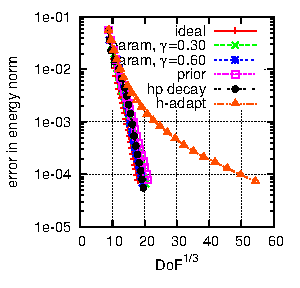
\includegraphics[width=1.15\textwidth]{hp_conv_E_1.pdf}}
\end{figure}
\column{0.33\textwidth}
\begin{figure}[h] 	
\centerline{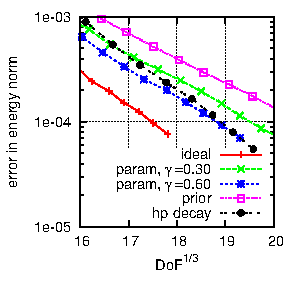
\includegraphics[width=1.15\textwidth]{hp_conv_E_2.pdf}}
\end{figure} 	
\column{0.33\textwidth}
\begin{figure}[h] 	
\centerline{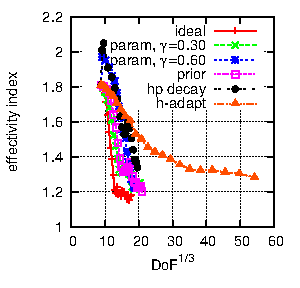
\includegraphics[width=1.15\textwidth]{hp_conv_E_3.pdf}}
\end{figure} 	
\end{columns}

\end{frame}

\begin{frame}
\frametitle{$hp$-refinement grids}

\begin{figure}
\hspace*{-0.4cm} {level 1}
\hspace{2cm} {level 5}
\hspace{2cm} {level 12}

\begin{center}
\hspace*{-0.5cm}\vertical{\hspace*{0.5cm} total view}
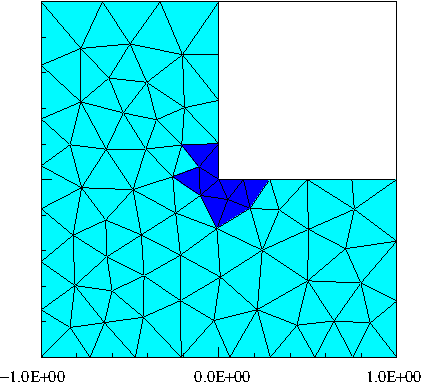
\includegraphics[height=0.27\textwidth]{case_E_hp_level1_T.pdf} \,
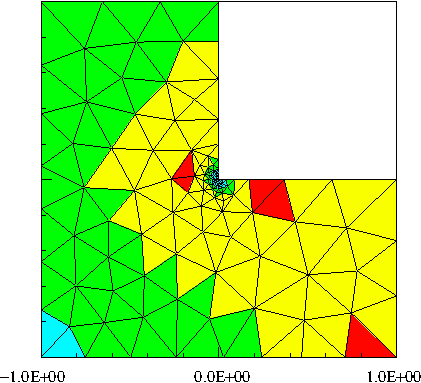
\includegraphics[height=0.27\textwidth]{case_E_hp_level5_T.pdf} \,
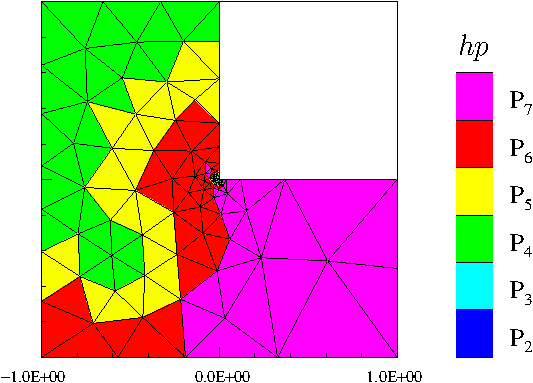
\includegraphics[height=0.27\textwidth]{case_E_hp_level12_T.pdf}

\vspace{2mm}

\hspace*{-0.5cm}\vertical{\hspace*{0.5cm}  zoom 10x}
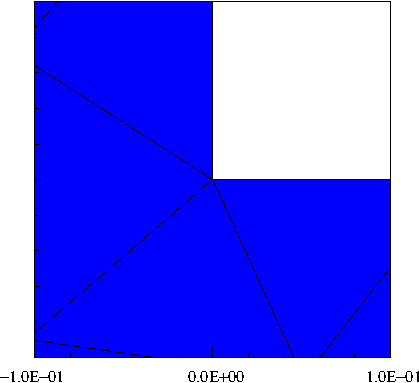
\includegraphics[height=0.27\textwidth]{case_E_hp_level1_D.pdf} \,
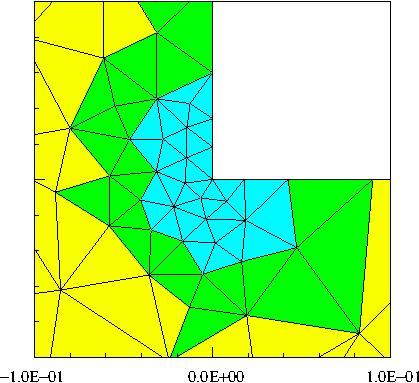
\includegraphics[height=0.27\textwidth]{case_E_hp_level5_D.pdf} \,
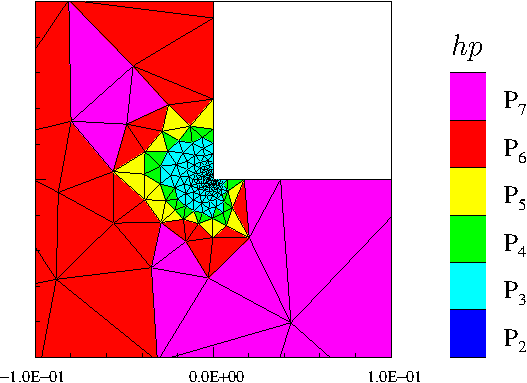
\includegraphics[height=0.27\textwidth]{case_E_hp_level12_D.pdf}
\vspace{2mm}

\end{center}
\end{figure}

\end{frame}
\section[Conclusion]{Conclusions and future directions}

\begin{frame}
\frametitle{Conclusions and future directions}

{\bf Conclusions}

\bi

\item \cblue{stability} of the \cblue{best piecewise polynomial
approximation}

\item \cblue{polynomial-degree-robust} local efficiency of \cblue{a
posteriori} error \cblue{estimates}

\item a \cblue{framework} covering all standard numerical methods (conforming
FEs, nonconforming FEs, discontinuous Galerkin, mixed FEs \ldots)

\ei

\pause

{\bf Ongoing generalizations}

\bi

\item transmission problems with sing changing coefficients

\item singularly-perturbed reaction-diffusion problems

\item Stokes equation

\item eigenvalue problems

\item heat equation

\ei

\end{frame}

\begin{frame}
    \frametitle{Bibliography}

    \vspace{-0.25cm}

    \begin{itemize}

    \item {\sc Ern A., Vohral\'\i k M.}, Stable broken $H^1$ and $\tH(\dv)$
    polynomial extensions for polynomial-degree-robust potential and flux
    reconstruction in three space dimensions, to be sumbitted, 2016.

    \item {\sc Ern A., Vohral\'\i k M.}, Polynomial-degree-robust a
    posteriori estimates in a unified setting for conforming,
    nonconforming, discontinuous Galerkin, and mixed discretizations, {\em
    SIAM J. Numer. Anal.}, {\bf 53} (2015), 1058--1081.

    \item {\sc Dolej\v s\'i V., Ern A., Vohral\'\i k M.}, $hp$-adaptation
    driven by polynomial-degree-robust a posteriori error estimates for
    elliptic problems, {\em SIAM J. Sci. Comput.}, accepted for
    publication, 2016.


    \end{itemize}

    \medskip
    \centerline{\cblue{\Large \bf Thank you for your attention!}}

\end{frame}

\end{document}
